\documentclass[a4paper,14pt]{extarticle}

\usepackage{float}
\usepackage{multirow}
\usepackage[utf8]{inputenc}
\usepackage[T1]{fontenc}
\usepackage[english,russian]{babel}
\usepackage{graphicx}
\usepackage{amsmath}
\usepackage{amssymb}
\usepackage{physics}
\usepackage[left=2cm, top=2cm, right=2cm, bottom=2cm]{geometry}
\usepackage{wrapfig}
\usepackage{subcaption}
% \setlength{\parindent}{0pt}
% \renewcommand{\arraystretch}{1.5}
\usepackage[unicode=true,colorlinks=true]{hyperref} % Гиперссылки

\title{\huge \textbf{ПРОЕКТНОЕ ПРЕДЛОЖЕНИЕ}\\\large VFD-часы со световым будильником}
%\author{\small Белокопытов Александр (Б01-507), Мартынов Александр (Б01-505)}
\date{}

\begin{document}

\maketitle

\section{Менторы:}

\begin{itemize}
	\item Тавитов Азамат Георгиевич
	\item Негодяев Андрей Сергеевич
\end{itemize}


\section{Команда:}

\begin{itemize}
	\item Мартынов Александр, группа Б01-505\\
	Email:
	\href{mailto:martynov.aleksandr@phystech.edu}{martynov.aleksandr@phystech.edu}\\
	Telegram:
	\href{https://t.me/mart_alx}{@mart\_alx}

	\item Белокопытов Александр, группа Б01-507\\
	Email:
	\href{mailto:belokopytov.aa@phystech.edu}{belokopytov.aa@phystech.edu}\\
	Telegram:
	\href{https://t.me/Werenter}{@Werenter}	
\end{itemize}

\section{Цель проекта и описание функционала:}

\subsection{Критический функционал}

Создаваемое устройство должно удоволетворять следующим требованиям:
\begin{itemize}
	\item
		Часы обладают двумя VFD дисплеями, способны отображать
		текущее время и дату
	\item
		Часы способны работать как будильник,
		издавая звуковой сигнал в заданное время
	\item
		Часы не должны останавливаться (сбрасываться)
		при отключении электропитания
	\item
		Часы собраны в корпусе, изготовленном например при
		помощи 3d печати (примерные габариты 170x100x90)
	\item
		Кнопки для настройки времени и будильника.
\end{itemize}

\subsection{Опциональная часть}

Также планируется следующий дополнительный функционал:
\begin{itemize}
	\item
		Измерение температуры от -40 до +80 $^\circ$C
		и влажности от 0 до 99\% (выбор диапазона обусловлен
		используемым датчиком)
	\item
		Лампа (дополнительный модуль), связывающаяся с 
		основным модулем по Wi-Fi, которая способствует
		более легкому пробуждению (опционально: с настраиваемой
		подсветкой)
	\item
		Синхронизация времени по сети
	\item
		Корпус, изготовленный из цельной древесины 
		(примерные габариты 170x100x90, примерно такие же, как и у прототипа)
\end{itemize}

% TODO: опциональная часть
% TODO: 170x100x90
% Питание 5В (адаптер)
% Диапазон температуры -40 +80 pm 0.5, влажность 0-99% pm 2%
%	Обоснование --- датчик
% Бюджет 700+800+600+1200      +500
%       ив18 уи4 esp32 плата   корпус
% Лампа 600+ 500 + 500 + 500
%      esp  корпус лента мелочевка
% Итог: 3800 + 2100 = 5900

% Заимствуем: dcdc power suply от alexgyver, аналог тоже
% ссылки https://www.kickstarter.com/projects/4059457/cybertube-a-vfd-clock-for-a-cyber-world
% https://alexgyver.ru/nixieclock/
% Идея делать vfd часы

% BASE: esp32 + displays + 74hc595+uln2003a + ps 5v + dcdc + temp
% Потенциал фабрика принтер, лазер, фрезер, фрезер ПП
% План

%Создать часы на основе вакуумно-люминисцентных (VFD)
%индикаторов, которые будут обладать следующим функционалом:
%\begin{itemize}
%	\item Отображение текущего времени (ч:мин)
%	\item Отображение даты (дд.мм.гггг или дд-мм-гг)
%	\item Отображение температуры и относительной влажности
%	\item Таймер и секундомер
%	\item Световой и звуковой будильник*
%	\item Автоматическая синхронизация времени по сети
%\end{itemize}

%(*) Световой будильник подразумевает наличие отдельного модуля
%(лампы), подключающегося к основному модулю (часам) по Wi-Fi.

% и еще чтобы дедлайны присутствовали

\section{Анализ существующих аналогов:}

Проект был вдохновлен существующими его аналогами:
\begin{itemize}
	\item
		Часы на индикаторе ИВ-18
		(рис. \ref{fig:vfd_analog})
		\url{https://www.kickstarter.com/projects/4059457/cybertube-a-vfd-clock-for-a-cyber-world}
	\item
		Часы на неоновых индикаторах
		(рис. \ref{fig:nixie_analog})
		\url{https://alexgyver.ru/nixieclock}
\end{itemize}

\begin{figure}[H]
	\centering

	\begin{subfigure}{0.5\linewidth}
		\centering
		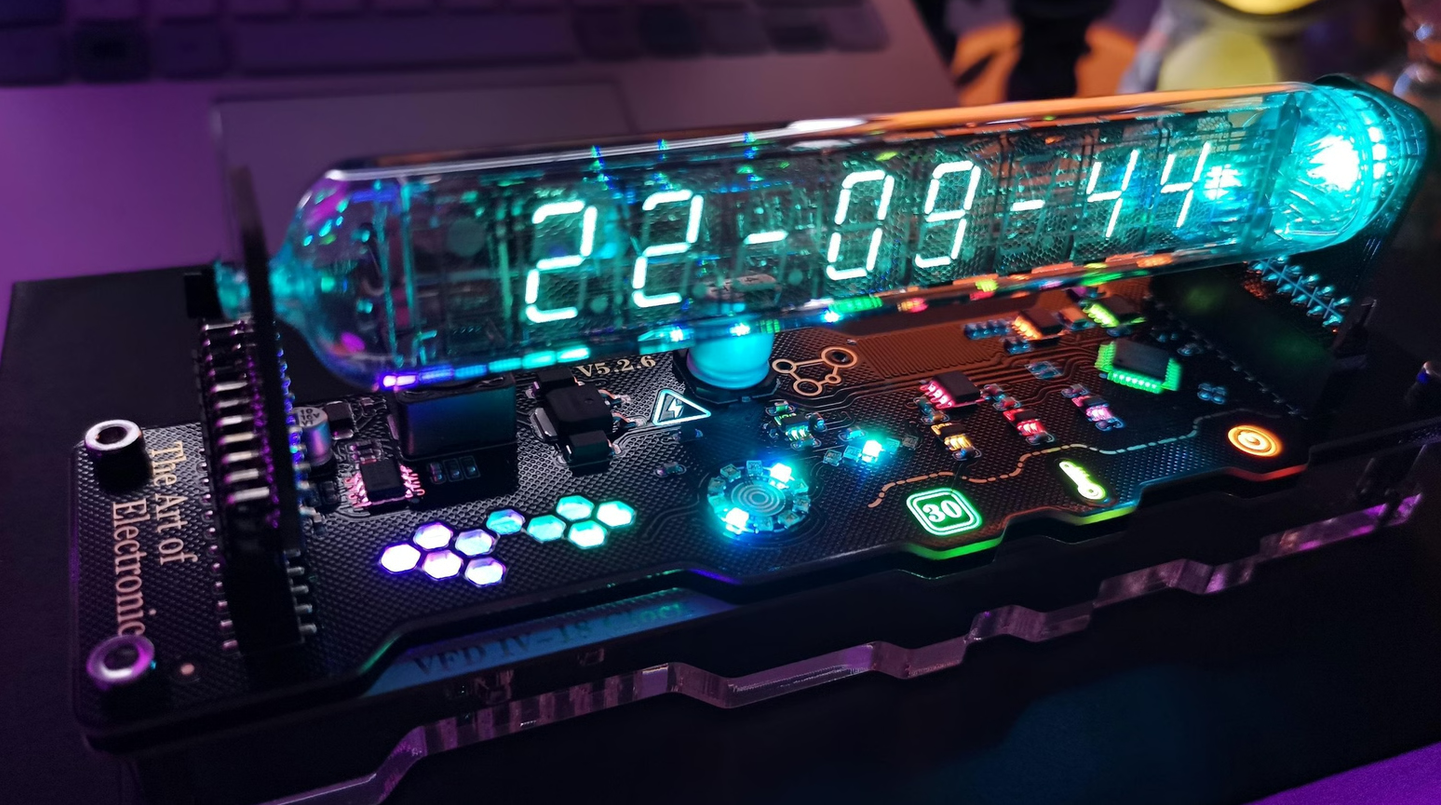
\includegraphics[width=0.7\linewidth]{images/vfd_analog.png}
		\caption{VFD-аналог}\label{fig:vfd_analog}
	\end{subfigure}%
	\begin{subfigure}{0.5\linewidth}
		\centering
		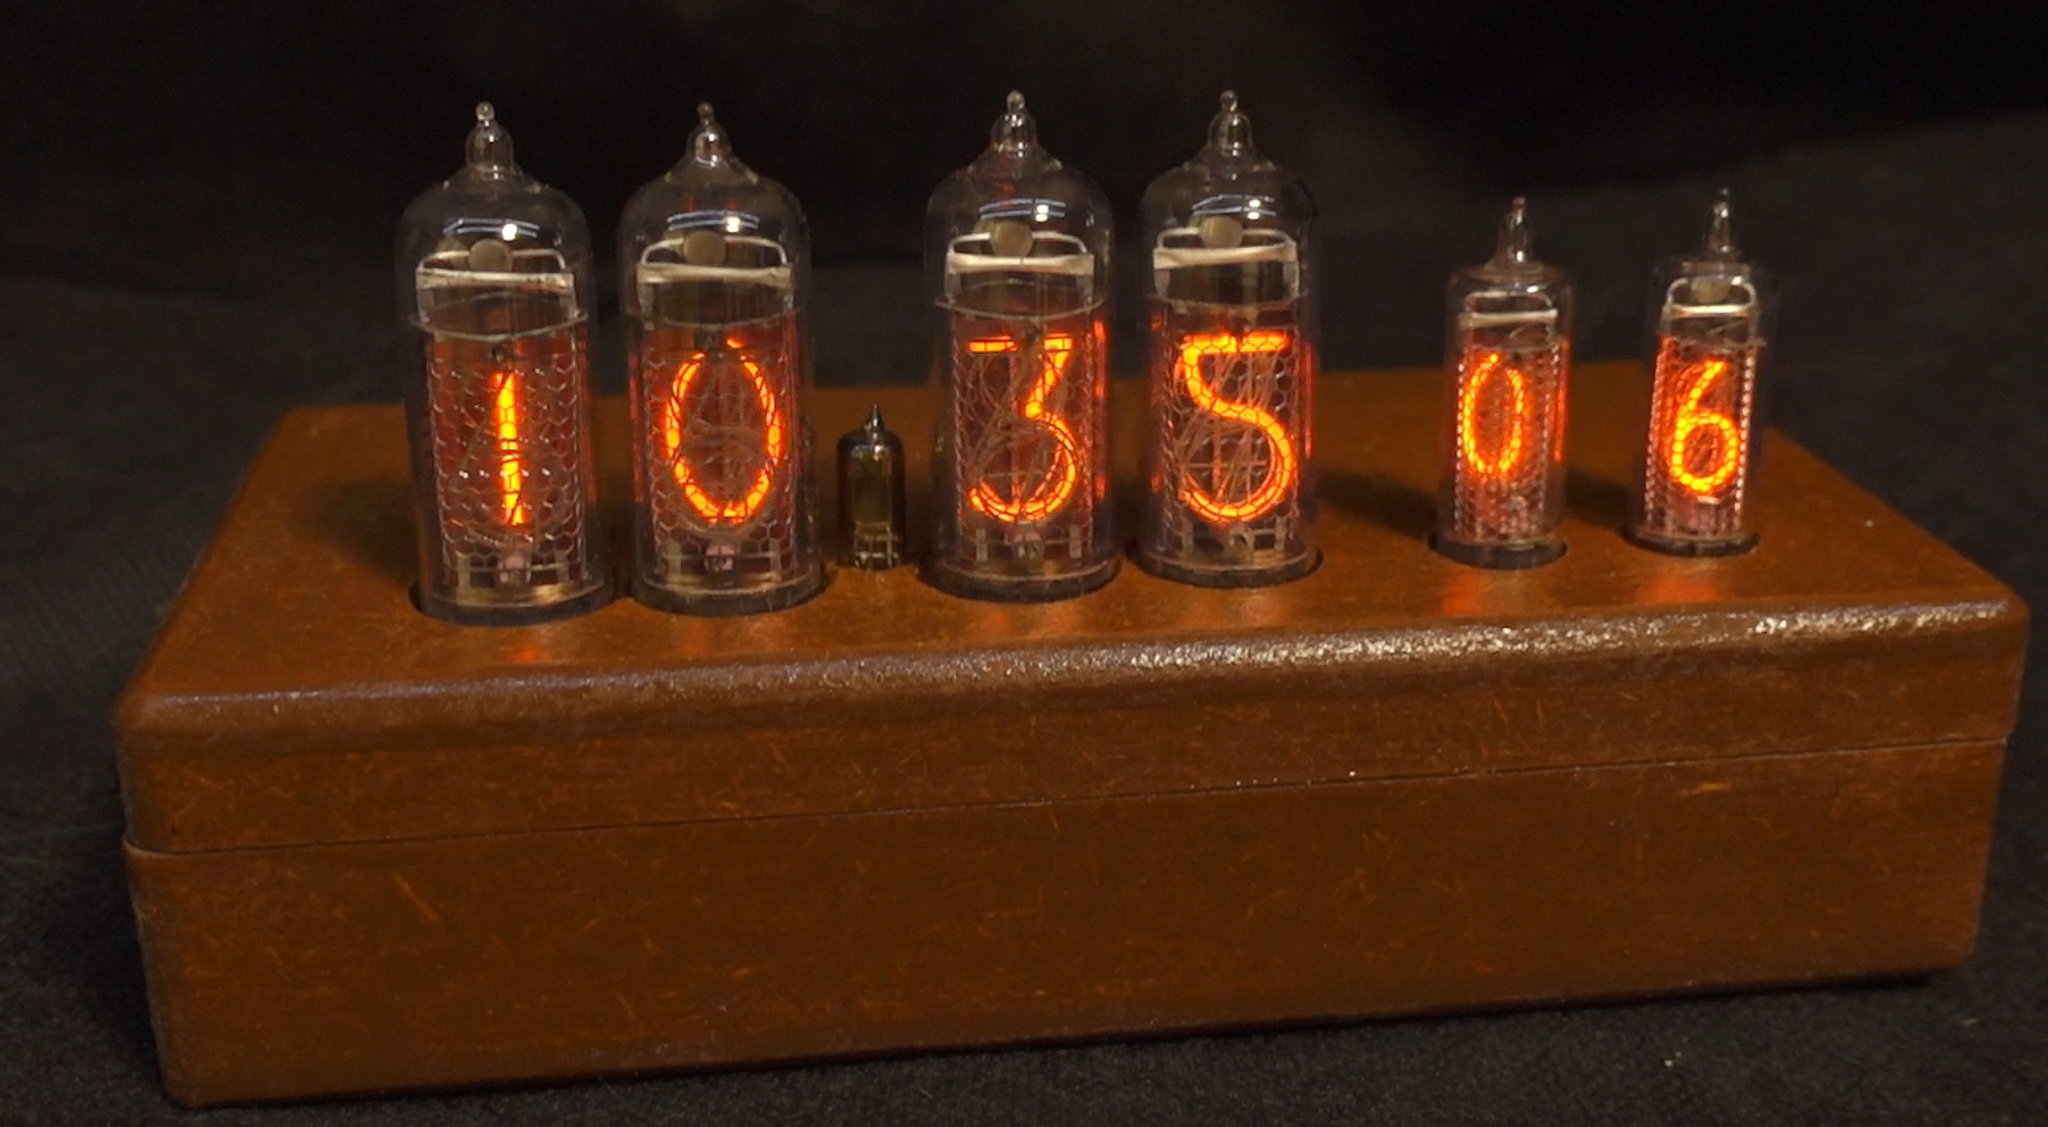
\includegraphics[width=0.7\linewidth]{images/nixie_analog.png}
		\caption{Nixie-аналог}\label{fig:nixie_analog}
	\end{subfigure}

	\caption{Анализ существующих аналогов}
\end{figure}

Два дисплея делают более удобным чтение времени, даты и температуры.
Выбор VFD индикаторов в качестве дисплеев обусловлен эстетическими
соображениями.

Из проекта nixieclock позаимствована идея повышающего DC-DC
преобразователя с генератором ШИМ от микроконтроллера. Такая
конструкция позволяет не ставить отдельный модуль DC-DC преобразователя.
Плюс такого решения в отсутствии необходимости ставить отдельный модуль питания,
которые на нужное для питания напряжение обладают сильно избыточной мощностью,
а соответственно и большим размером.

Реализация будильника-рассвета как отдельного модуля позволяет
независимо размещать лампу и сами часы.

\section{Эскиз проекта}
\begin{figure}[H]
	\begin{subfigure}{0.5\linewidth}
		\centering
		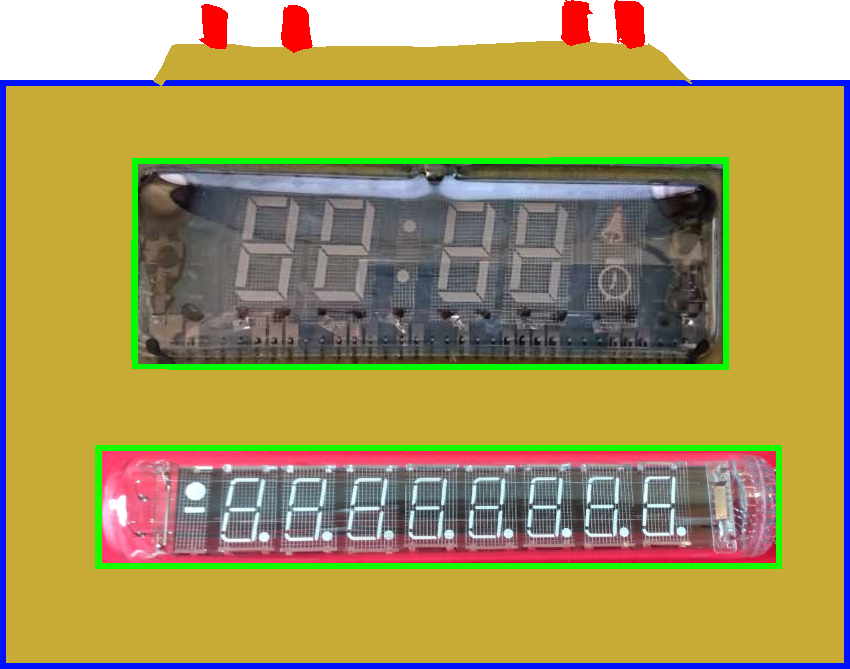
\includegraphics[width=0.5\linewidth]{images/draft.pdf}
		\caption{Основной блок}
	\end{subfigure}%
	\begin{subfigure}{0.5\linewidth}
		\centering
		
\includegraphics[width=0.2\linewidth]{images/lamp.pdf}
		\caption{Эскиз лампы}
	\end{subfigure}
\end{figure}



\section{Элементная база:}
\begin{itemize}
	\item Микроконтроллер ESP32
	\item ВЛИ ИЛЦ8-4/7Л (верхний дисплей)
	\item ВЛИ ИВЛ-18 (нижний дисплей)
	\item Драйвер (пары Дарлингтона ULN2003A)
	\item Преобразователь для питания индикаторов
	\item Микросхема RTC
	\item Датчики температуры и влажности
	\item Блок питания
	\item Светодиодная лента для лампы
\end{itemize}

\section{Бюджет}

Примерный бюджет часов и лампы составляет 3800 и 2100 рублей 
соответственно.

\section{Блок-схема}
\begin{figure}[H]
	\centering
	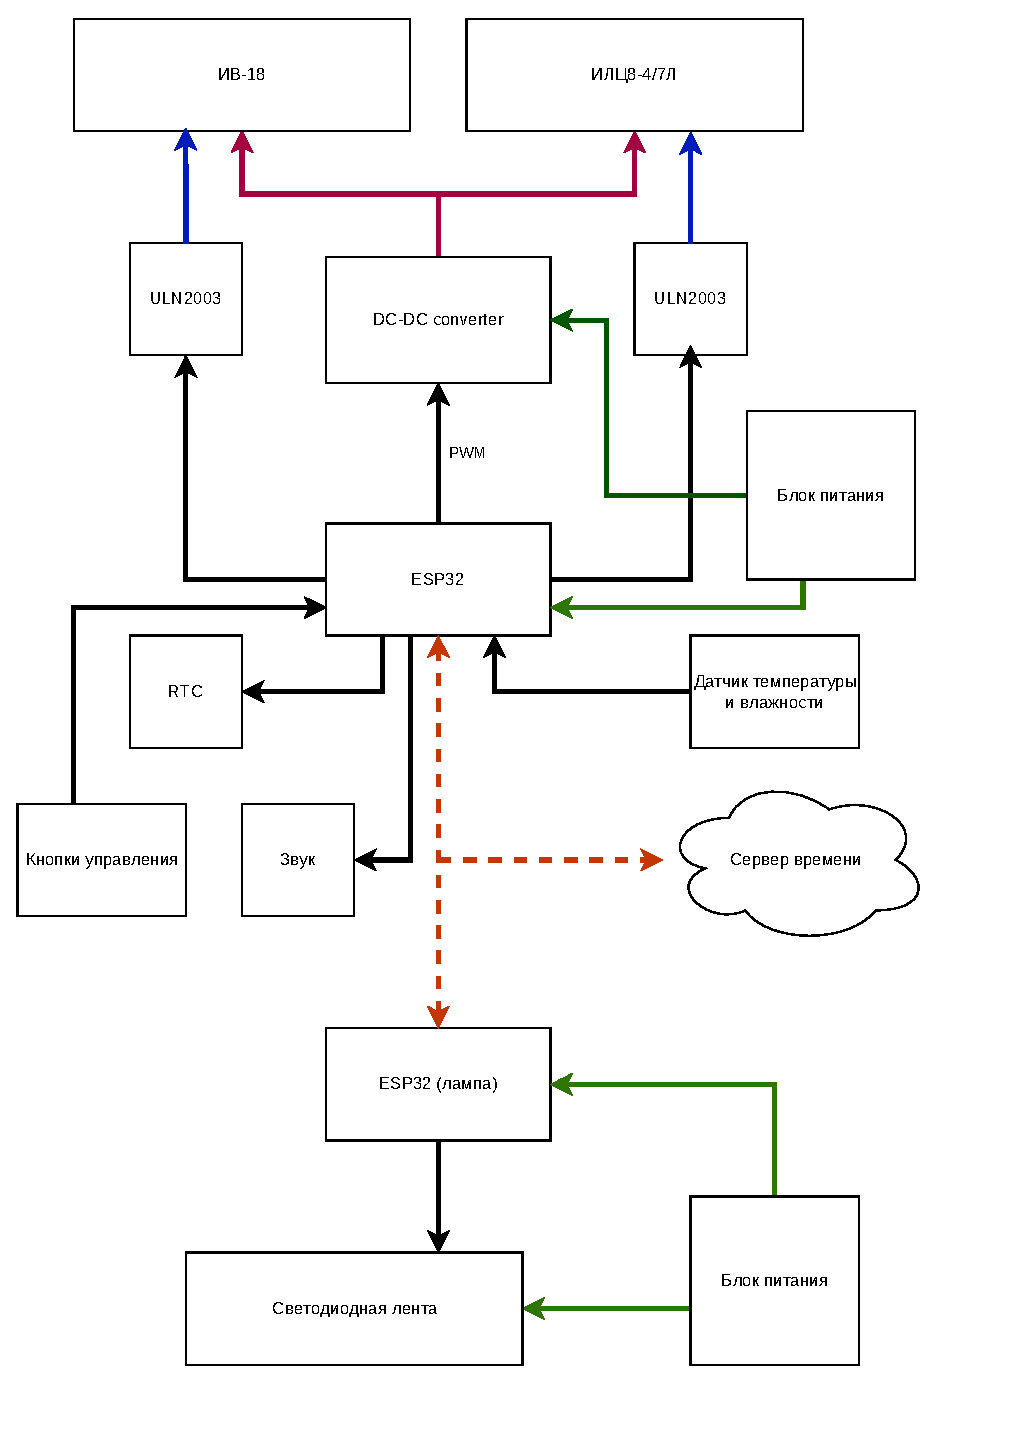
\includegraphics[width=0.9\textwidth]{images/block_schemev2.pdf}
	\caption{Блок-схема проекта}
\end{figure}

\section{План и задачи}

\subsection{Задачи проекта:}
\begin{enumerate}
	\item Выбор доступной элементной базы
	\item Создание CAD модели корпуса устройства
	\item Проектирование схемы часов
	\item Разводка печатной платы
	\item Программирование микроконтроллера
	\item Сборка и отладка устройства
\end{enumerate}

\subsection{План выполнения проекта:}
\begin{enumerate}
	\item [07.09] Актуализировать ПП
	\item [7.09-13.09] Собрать прототип преобразователя питания на макетной плате
	\item [14.09-20.09] Спроектировать и изготовить плату для прототипа
	\item [21.09-27.09] Запустить дисплеи
	\item [21.09-27.09] \textbf{Презентация РР, к этому моменту должна быть работоспособная схема дисплея}
	\item [28.09-04.10] Написать API для дисплея,
		собрать минимально рабочий прототип схемы,
		изготовить корпус на 3D принтере
	\item [05.10-11.10] Изготовить корпус из дерева и
		финальную плату
	\item [12.10-18.10] Собрать лампу (второй модуль)
	\item [19.10-31.10] Резерв, разработка опциональной части
	\item [19.10-25.10] \textbf{Презентация ППП, к этому моменту должен быть полностью готов прототип и желательно
		большая часть дополнительного функционала}
	\item [ноябрь] Резерв, полировка, подготовка к сдаче
	\item [07.12] \textbf{Итоговая презентация, к этому времени проект должен быть полностью готов}
\end{enumerate}


\end{document}
